% Created by tikzDevice version 0.7.0 on 2014-07-29 12:44:57
% !TEX encoding = UTF-8 Unicode
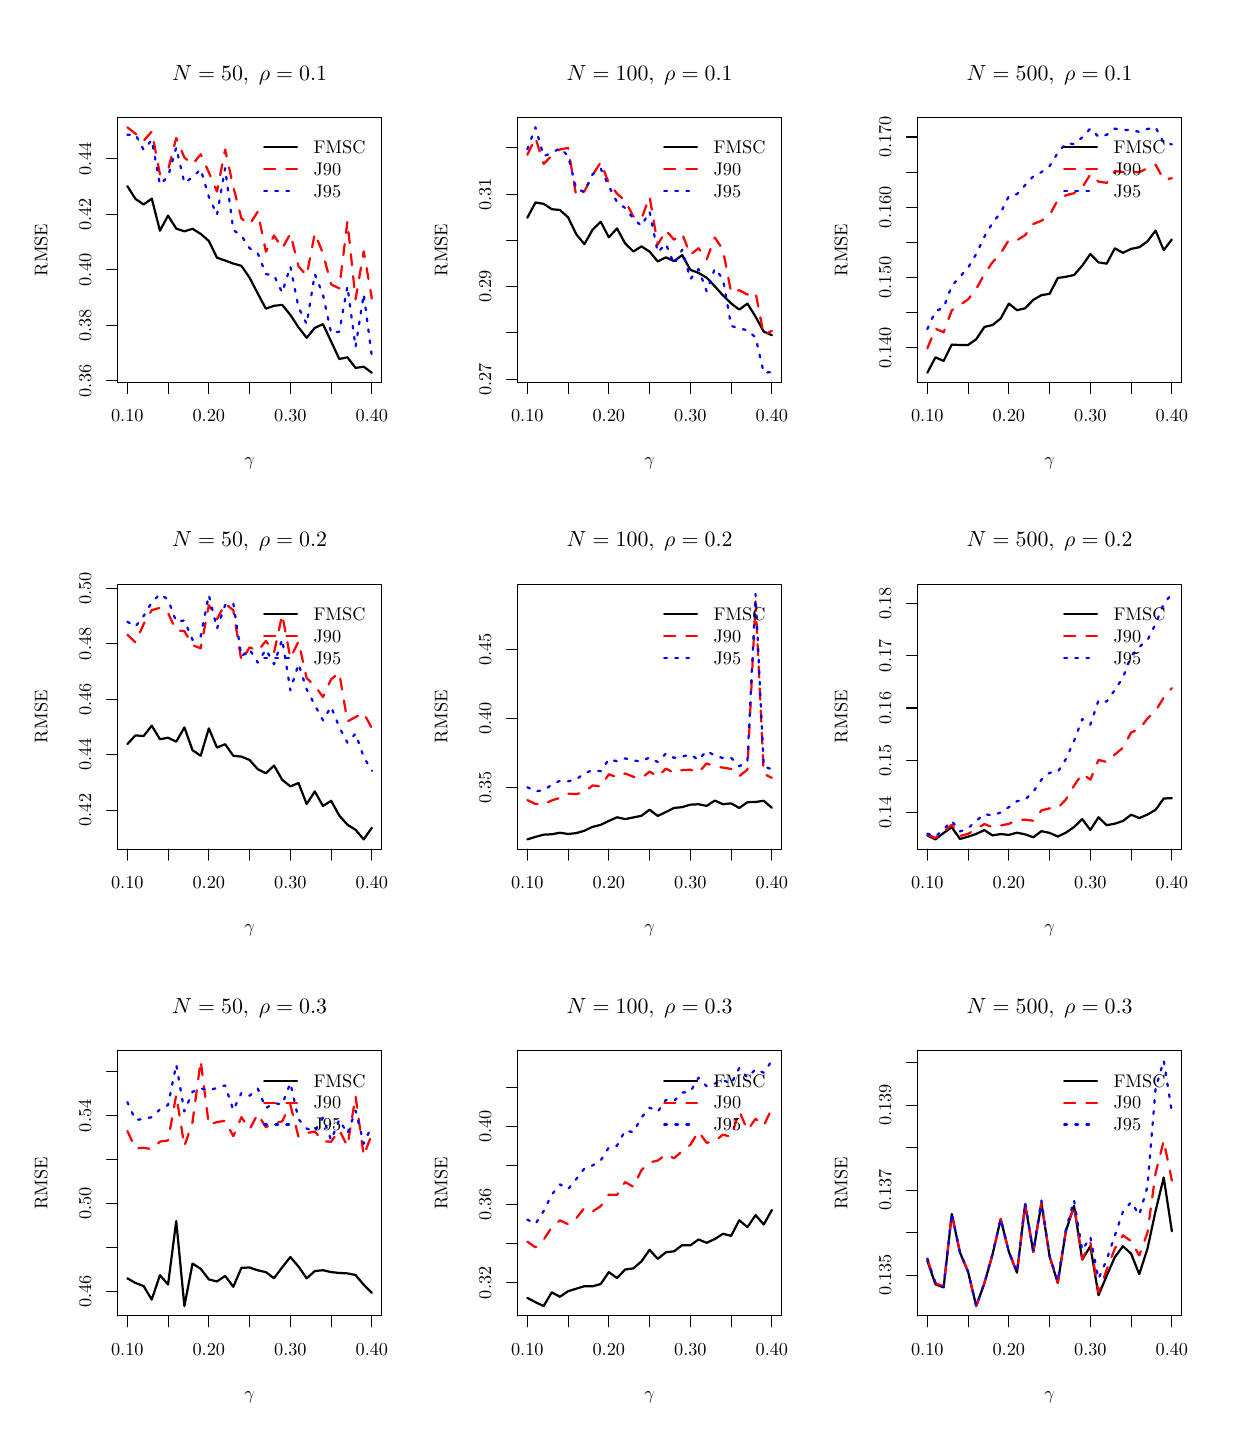
\begin{tikzpicture}[x=1pt,y=1pt]
\definecolor[named]{fillColor}{rgb}{1.00,1.00,1.00}
\path[use as bounding box,fill=fillColor,fill opacity=0.00] (0,0) rectangle (433.62,505.89);
\begin{scope}
\path[clip] ( 32.47,377.65) rectangle (127.91,473.42);
\definecolor[named]{drawColor}{rgb}{0.00,0.00,0.00}

\path[draw=drawColor,line width= 0.8pt,line join=round,line cap=round] ( 36.01,448.63) --
	( 38.95,444.01) --
	( 41.90,442.00) --
	( 44.84,444.12) --
	( 47.79,432.52) --
	( 50.73,437.99) --
	( 53.68,433.29) --
	( 56.63,432.29) --
	( 59.57,433.21) --
	( 62.52,431.36) --
	( 65.46,428.82) --
	( 68.41,422.77) --
	( 71.35,421.74) --
	( 74.30,420.65) --
	( 77.24,419.83) --
	( 80.19,415.53) --
	( 83.14,409.85) --
	( 86.08,404.35) --
	( 89.03,405.39) --
	( 91.97,405.71) --
	( 94.92,402.09) --
	( 97.86,397.62) --
	(100.81,393.82) --
	(103.75,397.39) --
	(106.70,398.77) --
	(109.65,392.51) --
	(112.59,386.15) --
	(115.54,386.77) --
	(118.48,382.94) --
	(121.43,383.38) --
	(124.37,381.20);
\end{scope}
\begin{scope}
\path[clip] (  0.00,  0.00) rectangle (433.62,505.89);
\definecolor[named]{drawColor}{rgb}{0.00,0.00,0.00}

\path[draw=drawColor,line width= 0.4pt,line join=round,line cap=round] ( 36.01,377.65) -- (124.37,377.65);

\path[draw=drawColor,line width= 0.4pt,line join=round,line cap=round] ( 36.01,377.65) -- ( 36.01,373.69);

\path[draw=drawColor,line width= 0.4pt,line join=round,line cap=round] ( 50.73,377.65) -- ( 50.73,373.69);

\path[draw=drawColor,line width= 0.4pt,line join=round,line cap=round] ( 65.46,377.65) -- ( 65.46,373.69);

\path[draw=drawColor,line width= 0.4pt,line join=round,line cap=round] ( 80.19,377.65) -- ( 80.19,373.69);

\path[draw=drawColor,line width= 0.4pt,line join=round,line cap=round] ( 94.92,377.65) -- ( 94.92,373.69);

\path[draw=drawColor,line width= 0.4pt,line join=round,line cap=round] (109.65,377.65) -- (109.65,373.69);

\path[draw=drawColor,line width= 0.4pt,line join=round,line cap=round] (124.37,377.65) -- (124.37,373.69);

\node[text=drawColor,anchor=base,inner sep=0pt, outer sep=0pt, scale=  0.66] at ( 36.01,363.40) {0.10};

\node[text=drawColor,anchor=base,inner sep=0pt, outer sep=0pt, scale=  0.66] at ( 65.46,363.40) {0.20};

\node[text=drawColor,anchor=base,inner sep=0pt, outer sep=0pt, scale=  0.66] at ( 94.92,363.40) {0.30};

\node[text=drawColor,anchor=base,inner sep=0pt, outer sep=0pt, scale=  0.66] at (124.37,363.40) {0.40};

\path[draw=drawColor,line width= 0.4pt,line join=round,line cap=round] ( 32.47,378.23) -- ( 32.47,458.47);

\path[draw=drawColor,line width= 0.4pt,line join=round,line cap=round] ( 32.47,378.23) -- ( 28.51,378.23);

\path[draw=drawColor,line width= 0.4pt,line join=round,line cap=round] ( 32.47,398.29) -- ( 28.51,398.29);

\path[draw=drawColor,line width= 0.4pt,line join=round,line cap=round] ( 32.47,418.35) -- ( 28.51,418.35);

\path[draw=drawColor,line width= 0.4pt,line join=round,line cap=round] ( 32.47,438.41) -- ( 28.51,438.41);

\path[draw=drawColor,line width= 0.4pt,line join=round,line cap=round] ( 32.47,458.47) -- ( 28.51,458.47);

\node[text=drawColor,rotate= 90.00,anchor=base,inner sep=0pt, outer sep=0pt, scale=  0.66] at ( 22.97,378.23) {0.36};

\node[text=drawColor,rotate= 90.00,anchor=base,inner sep=0pt, outer sep=0pt, scale=  0.66] at ( 22.97,398.29) {0.38};

\node[text=drawColor,rotate= 90.00,anchor=base,inner sep=0pt, outer sep=0pt, scale=  0.66] at ( 22.97,418.35) {0.40};

\node[text=drawColor,rotate= 90.00,anchor=base,inner sep=0pt, outer sep=0pt, scale=  0.66] at ( 22.97,438.41) {0.42};

\node[text=drawColor,rotate= 90.00,anchor=base,inner sep=0pt, outer sep=0pt, scale=  0.66] at ( 22.97,458.47) {0.44};

\path[draw=drawColor,line width= 0.4pt,line join=round,line cap=round] ( 32.47,377.65) --
	(127.91,377.65) --
	(127.91,473.42) --
	( 32.47,473.42) --
	( 32.47,377.65);
\end{scope}
\begin{scope}
\path[clip] (  0.00,337.26) rectangle (144.54,505.89);
\definecolor[named]{drawColor}{rgb}{0.00,0.00,0.00}

\node[text=drawColor,anchor=base,inner sep=0pt, outer sep=0pt, scale=  0.79] at ( 80.19,486.92) {\bfseries $N=50, \;\rho=0.1$};

\node[text=drawColor,anchor=base,inner sep=0pt, outer sep=0pt, scale=  0.66] at ( 80.19,347.56) {$\gamma$};

\node[text=drawColor,rotate= 90.00,anchor=base,inner sep=0pt, outer sep=0pt, scale=  0.66] at (  7.13,425.53) {RMSE};
\end{scope}
\begin{scope}
\path[clip] ( 32.47,377.65) rectangle (127.91,473.42);
\definecolor[named]{drawColor}{rgb}{1.00,0.00,0.00}

\path[draw=drawColor,line width= 0.8pt,dash pattern=on 4pt off 4pt ,line join=round,line cap=round] ( 36.01,469.87) --
	( 38.95,467.58) --
	( 41.90,465.00) --
	( 44.84,468.37) --
	( 47.79,452.93) --
	( 50.73,454.53) --
	( 53.68,466.01) --
	( 56.63,458.94) --
	( 59.57,456.47) --
	( 62.52,460.13) --
	( 65.46,453.62) --
	( 68.41,446.65) --
	( 71.35,461.84) --
	( 74.30,448.39) --
	( 77.24,436.94) --
	( 80.19,434.83) --
	( 83.14,439.35) --
	( 86.08,424.92) --
	( 89.03,430.80) --
	( 91.97,426.12) --
	( 94.92,431.46) --
	( 97.86,419.63) --
	(100.81,416.31) --
	(103.75,431.60) --
	(106.70,424.32) --
	(109.65,413.12) --
	(112.59,411.69) --
	(115.54,435.81) --
	(118.48,407.78) --
	(121.43,425.05) --
	(124.37,408.03);
\definecolor[named]{drawColor}{rgb}{0.00,0.00,1.00}

\path[draw=drawColor,line width= 0.8pt,dash pattern=on 1pt off 3pt ,line join=round,line cap=round] ( 36.01,467.15) --
	( 38.95,467.27) --
	( 41.90,461.76) --
	( 44.84,465.31) --
	( 47.79,449.15) --
	( 50.73,452.13) --
	( 53.68,462.57) --
	( 56.63,449.76) --
	( 59.57,451.84) --
	( 62.52,454.74) --
	( 65.46,444.76) --
	( 68.41,438.23) --
	( 71.35,455.13) --
	( 74.30,432.71) --
	( 77.24,430.76) --
	( 80.19,426.19) --
	( 83.14,424.37) --
	( 86.08,416.84) --
	( 89.03,416.37) --
	( 91.97,410.15) --
	( 94.92,419.58) --
	( 97.86,404.85) --
	(100.81,398.81) --
	(103.75,416.84) --
	(106.70,409.46) --
	(109.65,395.53) --
	(112.59,396.04) --
	(115.54,412.43) --
	(118.48,390.50) --
	(121.43,409.66) --
	(124.37,387.02);
\definecolor[named]{drawColor}{rgb}{0.00,0.00,0.00}

\path[draw=drawColor,line width= 0.8pt,line join=round,line cap=round] ( 85.47,462.63) -- ( 97.35,462.63);
\definecolor[named]{drawColor}{rgb}{1.00,0.00,0.00}

\path[draw=drawColor,line width= 0.8pt,dash pattern=on 4pt off 4pt ,line join=round,line cap=round] ( 85.47,454.71) -- ( 97.35,454.71);
\definecolor[named]{drawColor}{rgb}{0.00,0.00,1.00}

\path[draw=drawColor,line width= 0.8pt,dash pattern=on 1pt off 3pt ,line join=round,line cap=round] ( 85.47,446.79) -- ( 97.35,446.79);
\definecolor[named]{drawColor}{rgb}{0.00,0.00,0.00}

\node[text=drawColor,anchor=base west,inner sep=0pt, outer sep=0pt, scale=  0.66] at (103.29,460.35) {FMSC};

\node[text=drawColor,anchor=base west,inner sep=0pt, outer sep=0pt, scale=  0.66] at (103.29,452.43) {J90};

\node[text=drawColor,anchor=base west,inner sep=0pt, outer sep=0pt, scale=  0.66] at (103.29,444.51) {J95};
\end{scope}
\begin{scope}
\path[clip] (177.01,377.65) rectangle (272.45,473.42);
\definecolor[named]{drawColor}{rgb}{0.00,0.00,0.00}

\path[draw=drawColor,line width= 0.8pt,line join=round,line cap=round] (180.55,437.20) --
	(183.49,442.71) --
	(186.44,442.23) --
	(189.38,440.29) --
	(192.33,440.00) --
	(195.27,437.37) --
	(198.22,431.25) --
	(201.17,427.65) --
	(204.11,432.86) --
	(207.06,435.75) --
	(210.00,430.13) --
	(212.95,433.32) --
	(215.89,427.95) --
	(218.84,425.02) --
	(221.78,426.84) --
	(224.73,424.97) --
	(227.68,421.39) --
	(230.62,422.89) --
	(233.57,421.56) --
	(236.51,423.70) --
	(239.46,418.37) --
	(242.40,417.28) --
	(245.35,415.53) --
	(248.29,412.43) --
	(251.24,409.14) --
	(254.19,406.26) --
	(257.13,404.01) --
	(260.08,406.18) --
	(263.02,401.45) --
	(265.97,396.06) --
	(268.91,394.75);
\end{scope}
\begin{scope}
\path[clip] (  0.00,  0.00) rectangle (433.62,505.89);
\definecolor[named]{drawColor}{rgb}{0.00,0.00,0.00}

\path[draw=drawColor,line width= 0.4pt,line join=round,line cap=round] (180.55,377.65) -- (268.91,377.65);

\path[draw=drawColor,line width= 0.4pt,line join=round,line cap=round] (180.55,377.65) -- (180.55,373.69);

\path[draw=drawColor,line width= 0.4pt,line join=round,line cap=round] (195.27,377.65) -- (195.27,373.69);

\path[draw=drawColor,line width= 0.4pt,line join=round,line cap=round] (210.00,377.65) -- (210.00,373.69);

\path[draw=drawColor,line width= 0.4pt,line join=round,line cap=round] (224.73,377.65) -- (224.73,373.69);

\path[draw=drawColor,line width= 0.4pt,line join=round,line cap=round] (239.46,377.65) -- (239.46,373.69);

\path[draw=drawColor,line width= 0.4pt,line join=round,line cap=round] (254.19,377.65) -- (254.19,373.69);

\path[draw=drawColor,line width= 0.4pt,line join=round,line cap=round] (268.91,377.65) -- (268.91,373.69);

\node[text=drawColor,anchor=base,inner sep=0pt, outer sep=0pt, scale=  0.66] at (180.55,363.40) {0.10};

\node[text=drawColor,anchor=base,inner sep=0pt, outer sep=0pt, scale=  0.66] at (210.00,363.40) {0.20};

\node[text=drawColor,anchor=base,inner sep=0pt, outer sep=0pt, scale=  0.66] at (239.46,363.40) {0.30};

\node[text=drawColor,anchor=base,inner sep=0pt, outer sep=0pt, scale=  0.66] at (268.91,363.40) {0.40};

\path[draw=drawColor,line width= 0.4pt,line join=round,line cap=round] (177.01,378.90) -- (177.01,462.46);

\path[draw=drawColor,line width= 0.4pt,line join=round,line cap=round] (177.01,378.90) -- (173.05,378.90);

\path[draw=drawColor,line width= 0.4pt,line join=round,line cap=round] (177.01,395.61) -- (173.05,395.61);

\path[draw=drawColor,line width= 0.4pt,line join=round,line cap=round] (177.01,412.33) -- (173.05,412.33);

\path[draw=drawColor,line width= 0.4pt,line join=round,line cap=round] (177.01,429.04) -- (173.05,429.04);

\path[draw=drawColor,line width= 0.4pt,line join=round,line cap=round] (177.01,445.75) -- (173.05,445.75);

\path[draw=drawColor,line width= 0.4pt,line join=round,line cap=round] (177.01,462.46) -- (173.05,462.46);

\node[text=drawColor,rotate= 90.00,anchor=base,inner sep=0pt, outer sep=0pt, scale=  0.66] at (167.51,378.90) {0.27};

\node[text=drawColor,rotate= 90.00,anchor=base,inner sep=0pt, outer sep=0pt, scale=  0.66] at (167.51,412.33) {0.29};

\node[text=drawColor,rotate= 90.00,anchor=base,inner sep=0pt, outer sep=0pt, scale=  0.66] at (167.51,445.75) {0.31};

\path[draw=drawColor,line width= 0.4pt,line join=round,line cap=round] (177.01,377.65) --
	(272.45,377.65) --
	(272.45,473.42) --
	(177.01,473.42) --
	(177.01,377.65);
\end{scope}
\begin{scope}
\path[clip] (144.54,337.26) rectangle (289.08,505.89);
\definecolor[named]{drawColor}{rgb}{0.00,0.00,0.00}

\node[text=drawColor,anchor=base,inner sep=0pt, outer sep=0pt, scale=  0.79] at (224.73,486.92) {\bfseries $N=100, \;\rho=0.1$};

\node[text=drawColor,anchor=base,inner sep=0pt, outer sep=0pt, scale=  0.66] at (224.73,347.56) {$\gamma$};

\node[text=drawColor,rotate= 90.00,anchor=base,inner sep=0pt, outer sep=0pt, scale=  0.66] at (151.67,425.53) {RMSE};
\end{scope}
\begin{scope}
\path[clip] (177.01,377.65) rectangle (272.45,473.42);
\definecolor[named]{drawColor}{rgb}{1.00,0.00,0.00}

\path[draw=drawColor,line width= 0.8pt,dash pattern=on 4pt off 4pt ,line join=round,line cap=round] (180.55,459.93) --
	(183.49,466.08) --
	(186.44,456.64) --
	(189.38,459.68) --
	(192.33,461.89) --
	(195.27,462.44) --
	(198.22,445.10) --
	(201.17,446.72) --
	(204.11,452.55) --
	(207.06,457.26) --
	(210.00,449.72) --
	(212.95,445.93) --
	(215.89,443.39) --
	(218.84,437.71) --
	(221.78,436.89) --
	(224.73,444.78) --
	(227.68,427.45) --
	(230.62,432.63) --
	(233.57,429.26) --
	(236.51,431.42) --
	(239.46,423.82) --
	(242.40,426.18) --
	(245.35,422.11) --
	(248.29,430.04) --
	(251.24,425.62) --
	(254.19,410.16) --
	(257.13,411.02) --
	(260.08,409.44) --
	(263.02,410.19) --
	(265.97,394.84) --
	(268.91,396.32);
\definecolor[named]{drawColor}{rgb}{0.00,0.00,1.00}

\path[draw=drawColor,line width= 0.8pt,dash pattern=on 1pt off 3pt ,line join=round,line cap=round] (180.55,461.93) --
	(183.49,469.87) --
	(186.44,459.47) --
	(189.38,460.52) --
	(192.33,462.37) --
	(195.27,459.60) --
	(198.22,447.64) --
	(201.17,446.57) --
	(204.11,452.87) --
	(207.06,454.97) --
	(210.00,448.62) --
	(212.95,442.83) --
	(215.89,440.72) --
	(218.84,436.92) --
	(221.78,434.25) --
	(224.73,439.38) --
	(227.68,424.72) --
	(230.62,427.78) --
	(233.57,420.48) --
	(236.51,425.63) --
	(239.46,415.04) --
	(242.40,418.66) --
	(245.35,410.65) --
	(248.29,418.80) --
	(251.24,415.13) --
	(254.19,398.11) --
	(257.13,397.22) --
	(260.08,396.54) --
	(263.02,393.95) --
	(265.97,381.20) --
	(268.91,381.44);
\definecolor[named]{drawColor}{rgb}{0.00,0.00,0.00}

\path[draw=drawColor,line width= 0.8pt,line join=round,line cap=round] (230.01,462.63) -- (241.89,462.63);
\definecolor[named]{drawColor}{rgb}{1.00,0.00,0.00}

\path[draw=drawColor,line width= 0.8pt,dash pattern=on 4pt off 4pt ,line join=round,line cap=round] (230.01,454.71) -- (241.89,454.71);
\definecolor[named]{drawColor}{rgb}{0.00,0.00,1.00}

\path[draw=drawColor,line width= 0.8pt,dash pattern=on 1pt off 3pt ,line join=round,line cap=round] (230.01,446.79) -- (241.89,446.79);
\definecolor[named]{drawColor}{rgb}{0.00,0.00,0.00}

\node[text=drawColor,anchor=base west,inner sep=0pt, outer sep=0pt, scale=  0.66] at (247.83,460.35) {FMSC};

\node[text=drawColor,anchor=base west,inner sep=0pt, outer sep=0pt, scale=  0.66] at (247.83,452.43) {J90};

\node[text=drawColor,anchor=base west,inner sep=0pt, outer sep=0pt, scale=  0.66] at (247.83,444.51) {J95};
\end{scope}
\begin{scope}
\path[clip] (321.55,377.65) rectangle (416.99,473.42);
\definecolor[named]{drawColor}{rgb}{0.00,0.00,0.00}

\path[draw=drawColor,line width= 0.8pt,line join=round,line cap=round] (325.09,381.20) --
	(328.03,386.76) --
	(330.98,385.44) --
	(333.92,391.37) --
	(336.87,391.21) --
	(339.81,391.24) --
	(342.76,393.30) --
	(345.71,397.75) --
	(348.65,398.43) --
	(351.60,400.79) --
	(354.54,406.18) --
	(357.49,403.80) --
	(360.43,404.49) --
	(363.38,407.55) --
	(366.32,409.23) --
	(369.27,409.71) --
	(372.22,415.43) --
	(375.16,415.87) --
	(378.11,416.51) --
	(381.05,419.87) --
	(384.00,424.10) --
	(386.94,421.07) --
	(389.89,420.61) --
	(392.83,426.12) --
	(395.78,424.53) --
	(398.73,425.96) --
	(401.67,426.54) --
	(404.62,428.64) --
	(407.56,432.54) --
	(410.51,425.50) --
	(413.45,429.38);
\end{scope}
\begin{scope}
\path[clip] (  0.00,  0.00) rectangle (433.62,505.89);
\definecolor[named]{drawColor}{rgb}{0.00,0.00,0.00}

\path[draw=drawColor,line width= 0.4pt,line join=round,line cap=round] (325.09,377.65) -- (413.45,377.65);

\path[draw=drawColor,line width= 0.4pt,line join=round,line cap=round] (325.09,377.65) -- (325.09,373.69);

\path[draw=drawColor,line width= 0.4pt,line join=round,line cap=round] (339.81,377.65) -- (339.81,373.69);

\path[draw=drawColor,line width= 0.4pt,line join=round,line cap=round] (354.54,377.65) -- (354.54,373.69);

\path[draw=drawColor,line width= 0.4pt,line join=round,line cap=round] (369.27,377.65) -- (369.27,373.69);

\path[draw=drawColor,line width= 0.4pt,line join=round,line cap=round] (384.00,377.65) -- (384.00,373.69);

\path[draw=drawColor,line width= 0.4pt,line join=round,line cap=round] (398.73,377.65) -- (398.73,373.69);

\path[draw=drawColor,line width= 0.4pt,line join=round,line cap=round] (413.45,377.65) -- (413.45,373.69);

\node[text=drawColor,anchor=base,inner sep=0pt, outer sep=0pt, scale=  0.66] at (325.09,363.40) {0.10};

\node[text=drawColor,anchor=base,inner sep=0pt, outer sep=0pt, scale=  0.66] at (354.54,363.40) {0.20};

\node[text=drawColor,anchor=base,inner sep=0pt, outer sep=0pt, scale=  0.66] at (384.00,363.40) {0.30};

\node[text=drawColor,anchor=base,inner sep=0pt, outer sep=0pt, scale=  0.66] at (413.45,363.40) {0.40};

\path[draw=drawColor,line width= 0.4pt,line join=round,line cap=round] (321.55,390.23) -- (321.55,466.37);

\path[draw=drawColor,line width= 0.4pt,line join=round,line cap=round] (321.55,390.23) -- (317.59,390.23);

\path[draw=drawColor,line width= 0.4pt,line join=round,line cap=round] (321.55,402.92) -- (317.59,402.92);

\path[draw=drawColor,line width= 0.4pt,line join=round,line cap=round] (321.55,415.61) -- (317.59,415.61);

\path[draw=drawColor,line width= 0.4pt,line join=round,line cap=round] (321.55,428.30) -- (317.59,428.30);

\path[draw=drawColor,line width= 0.4pt,line join=round,line cap=round] (321.55,440.99) -- (317.59,440.99);

\path[draw=drawColor,line width= 0.4pt,line join=round,line cap=round] (321.55,453.68) -- (317.59,453.68);

\path[draw=drawColor,line width= 0.4pt,line join=round,line cap=round] (321.55,466.37) -- (317.59,466.37);

\node[text=drawColor,rotate= 90.00,anchor=base,inner sep=0pt, outer sep=0pt, scale=  0.66] at (312.05,390.23) {0.140};

\node[text=drawColor,rotate= 90.00,anchor=base,inner sep=0pt, outer sep=0pt, scale=  0.66] at (312.05,415.61) {0.150};

\node[text=drawColor,rotate= 90.00,anchor=base,inner sep=0pt, outer sep=0pt, scale=  0.66] at (312.05,440.99) {0.160};

\node[text=drawColor,rotate= 90.00,anchor=base,inner sep=0pt, outer sep=0pt, scale=  0.66] at (312.05,466.37) {0.170};

\path[draw=drawColor,line width= 0.4pt,line join=round,line cap=round] (321.55,377.65) --
	(416.99,377.65) --
	(416.99,473.42) --
	(321.55,473.42) --
	(321.55,377.65);
\end{scope}
\begin{scope}
\path[clip] (289.08,337.26) rectangle (433.62,505.89);
\definecolor[named]{drawColor}{rgb}{0.00,0.00,0.00}

\node[text=drawColor,anchor=base,inner sep=0pt, outer sep=0pt, scale=  0.79] at (369.27,486.92) {\bfseries $N=500, \;\rho=0.1$};

\node[text=drawColor,anchor=base,inner sep=0pt, outer sep=0pt, scale=  0.66] at (369.27,347.56) {$\gamma$};

\node[text=drawColor,rotate= 90.00,anchor=base,inner sep=0pt, outer sep=0pt, scale=  0.66] at (296.21,425.53) {RMSE};
\end{scope}
\begin{scope}
\path[clip] (321.55,377.65) rectangle (416.99,473.42);
\definecolor[named]{drawColor}{rgb}{1.00,0.00,0.00}

\path[draw=drawColor,line width= 0.8pt,dash pattern=on 4pt off 4pt ,line join=round,line cap=round] (325.09,389.98) --
	(328.03,397.10) --
	(330.98,395.79) --
	(333.92,403.74) --
	(336.87,405.67) --
	(339.81,407.69) --
	(342.76,411.44) --
	(345.71,416.86) --
	(348.65,421.13) --
	(351.60,424.37) --
	(354.54,429.18) --
	(357.49,429.09) --
	(360.43,430.91) --
	(363.38,434.94) --
	(366.32,436.13) --
	(369.27,438.13) --
	(372.22,443.64) --
	(375.16,445.31) --
	(378.11,446.08) --
	(381.05,448.10) --
	(384.00,452.88) --
	(386.94,450.25) --
	(389.89,449.80) --
	(392.83,454.05) --
	(395.78,453.76) --
	(398.73,453.80) --
	(401.67,453.59) --
	(404.62,455.15) --
	(407.56,456.39) --
	(410.51,451.02) --
	(413.45,451.46);
\definecolor[named]{drawColor}{rgb}{0.00,0.00,1.00}

\path[draw=drawColor,line width= 0.8pt,dash pattern=on 1pt off 3pt ,line join=round,line cap=round] (325.09,396.98) --
	(328.03,403.46) --
	(330.98,404.72) --
	(333.92,412.60) --
	(336.87,415.88) --
	(339.81,419.15) --
	(342.76,424.10) --
	(345.71,430.37) --
	(348.65,435.37) --
	(351.60,439.01) --
	(354.54,444.98) --
	(357.49,445.75) --
	(360.43,448.99) --
	(363.38,452.21) --
	(366.32,453.68) --
	(369.27,455.86) --
	(372.22,460.65) --
	(375.16,464.03) --
	(378.11,463.85) --
	(381.05,466.22) --
	(384.00,469.43) --
	(386.94,466.48) --
	(389.89,467.15) --
	(392.83,469.41) --
	(395.78,468.90) --
	(398.73,468.90) --
	(401.67,468.22) --
	(404.62,469.25) --
	(407.56,469.87) --
	(410.51,464.23) --
	(413.45,463.72);
\definecolor[named]{drawColor}{rgb}{0.00,0.00,0.00}

\path[draw=drawColor,line width= 0.8pt,line join=round,line cap=round] (374.55,462.63) -- (386.43,462.63);
\definecolor[named]{drawColor}{rgb}{1.00,0.00,0.00}

\path[draw=drawColor,line width= 0.8pt,dash pattern=on 4pt off 4pt ,line join=round,line cap=round] (374.55,454.71) -- (386.43,454.71);
\definecolor[named]{drawColor}{rgb}{0.00,0.00,1.00}

\path[draw=drawColor,line width= 0.8pt,dash pattern=on 1pt off 3pt ,line join=round,line cap=round] (374.55,446.79) -- (386.43,446.79);
\definecolor[named]{drawColor}{rgb}{0.00,0.00,0.00}

\node[text=drawColor,anchor=base west,inner sep=0pt, outer sep=0pt, scale=  0.66] at (392.37,460.35) {FMSC};

\node[text=drawColor,anchor=base west,inner sep=0pt, outer sep=0pt, scale=  0.66] at (392.37,452.43) {J90};

\node[text=drawColor,anchor=base west,inner sep=0pt, outer sep=0pt, scale=  0.66] at (392.37,444.51) {J95};
\end{scope}
\begin{scope}
\path[clip] ( 32.47,209.02) rectangle (127.91,304.79);
\definecolor[named]{drawColor}{rgb}{0.00,0.00,0.00}

\path[draw=drawColor,line width= 0.8pt,line join=round,line cap=round] ( 36.01,247.00) --
	( 38.95,250.15) --
	( 41.90,249.93) --
	( 44.84,253.66) --
	( 47.79,248.77) --
	( 50.73,249.31) --
	( 53.68,247.88) --
	( 56.63,253.03) --
	( 59.57,244.79) --
	( 62.52,242.80) --
	( 65.46,252.68) --
	( 68.41,245.76) --
	( 71.35,246.96) --
	( 74.30,242.79) --
	( 77.24,242.49) --
	( 80.19,241.26) --
	( 83.14,237.94) --
	( 86.08,236.47) --
	( 89.03,239.24) --
	( 91.97,234.11) --
	( 94.92,231.72) --
	( 97.86,232.94) --
	(100.81,225.35) --
	(103.75,229.91) --
	(106.70,224.62) --
	(109.65,226.52) --
	(112.59,221.19) --
	(115.54,217.88) --
	(118.48,216.05) --
	(121.43,212.57) --
	(124.37,216.78);
\end{scope}
\begin{scope}
\path[clip] (  0.00,  0.00) rectangle (433.62,505.89);
\definecolor[named]{drawColor}{rgb}{0.00,0.00,0.00}

\path[draw=drawColor,line width= 0.4pt,line join=round,line cap=round] ( 36.01,209.02) -- (124.37,209.02);

\path[draw=drawColor,line width= 0.4pt,line join=round,line cap=round] ( 36.01,209.02) -- ( 36.01,205.06);

\path[draw=drawColor,line width= 0.4pt,line join=round,line cap=round] ( 50.73,209.02) -- ( 50.73,205.06);

\path[draw=drawColor,line width= 0.4pt,line join=round,line cap=round] ( 65.46,209.02) -- ( 65.46,205.06);

\path[draw=drawColor,line width= 0.4pt,line join=round,line cap=round] ( 80.19,209.02) -- ( 80.19,205.06);

\path[draw=drawColor,line width= 0.4pt,line join=round,line cap=round] ( 94.92,209.02) -- ( 94.92,205.06);

\path[draw=drawColor,line width= 0.4pt,line join=round,line cap=round] (109.65,209.02) -- (109.65,205.06);

\path[draw=drawColor,line width= 0.4pt,line join=round,line cap=round] (124.37,209.02) -- (124.37,205.06);

\node[text=drawColor,anchor=base,inner sep=0pt, outer sep=0pt, scale=  0.66] at ( 36.01,194.77) {0.10};

\node[text=drawColor,anchor=base,inner sep=0pt, outer sep=0pt, scale=  0.66] at ( 65.46,194.77) {0.20};

\node[text=drawColor,anchor=base,inner sep=0pt, outer sep=0pt, scale=  0.66] at ( 94.92,194.77) {0.30};

\node[text=drawColor,anchor=base,inner sep=0pt, outer sep=0pt, scale=  0.66] at (124.37,194.77) {0.40};

\path[draw=drawColor,line width= 0.4pt,line join=round,line cap=round] ( 32.47,223.17) -- ( 32.47,303.24);

\path[draw=drawColor,line width= 0.4pt,line join=round,line cap=round] ( 32.47,223.17) -- ( 28.51,223.17);

\path[draw=drawColor,line width= 0.4pt,line join=round,line cap=round] ( 32.47,243.18) -- ( 28.51,243.18);

\path[draw=drawColor,line width= 0.4pt,line join=round,line cap=round] ( 32.47,263.20) -- ( 28.51,263.20);

\path[draw=drawColor,line width= 0.4pt,line join=round,line cap=round] ( 32.47,283.22) -- ( 28.51,283.22);

\path[draw=drawColor,line width= 0.4pt,line join=round,line cap=round] ( 32.47,303.24) -- ( 28.51,303.24);

\node[text=drawColor,rotate= 90.00,anchor=base,inner sep=0pt, outer sep=0pt, scale=  0.66] at ( 22.97,223.17) {0.42};

\node[text=drawColor,rotate= 90.00,anchor=base,inner sep=0pt, outer sep=0pt, scale=  0.66] at ( 22.97,243.18) {0.44};

\node[text=drawColor,rotate= 90.00,anchor=base,inner sep=0pt, outer sep=0pt, scale=  0.66] at ( 22.97,263.20) {0.46};

\node[text=drawColor,rotate= 90.00,anchor=base,inner sep=0pt, outer sep=0pt, scale=  0.66] at ( 22.97,283.22) {0.48};

\node[text=drawColor,rotate= 90.00,anchor=base,inner sep=0pt, outer sep=0pt, scale=  0.66] at ( 22.97,303.24) {0.50};

\path[draw=drawColor,line width= 0.4pt,line join=round,line cap=round] ( 32.47,209.02) --
	(127.91,209.02) --
	(127.91,304.79) --
	( 32.47,304.79) --
	( 32.47,209.02);
\end{scope}
\begin{scope}
\path[clip] (  0.00,168.63) rectangle (144.54,337.26);
\definecolor[named]{drawColor}{rgb}{0.00,0.00,0.00}

\node[text=drawColor,anchor=base,inner sep=0pt, outer sep=0pt, scale=  0.79] at ( 80.19,318.29) {\bfseries $N=50, \;\rho=0.2$};

\node[text=drawColor,anchor=base,inner sep=0pt, outer sep=0pt, scale=  0.66] at ( 80.19,178.93) {$\gamma$};

\node[text=drawColor,rotate= 90.00,anchor=base,inner sep=0pt, outer sep=0pt, scale=  0.66] at (  7.13,256.90) {RMSE};
\end{scope}
\begin{scope}
\path[clip] ( 32.47,209.02) rectangle (127.91,304.79);
\definecolor[named]{drawColor}{rgb}{1.00,0.00,0.00}

\path[draw=drawColor,line width= 0.8pt,dash pattern=on 4pt off 4pt ,line join=round,line cap=round] ( 36.01,286.57) --
	( 38.95,283.76) --
	( 41.90,290.37) --
	( 44.84,295.43) --
	( 47.79,296.23) --
	( 50.73,294.33) --
	( 53.68,288.08) --
	( 56.63,287.82) --
	( 59.57,282.75) --
	( 62.52,281.62) --
	( 65.46,297.18) --
	( 68.41,292.12) --
	( 71.35,297.79) --
	( 74.30,295.35) --
	( 77.24,277.00) --
	( 80.19,281.97) --
	( 83.14,280.69) --
	( 86.08,284.28) --
	( 89.03,280.11) --
	( 91.97,293.78) --
	( 94.92,278.08) --
	( 97.86,284.04) --
	(100.81,270.85) --
	(103.75,268.09) --
	(106.70,264.02) --
	(109.65,270.45) --
	(112.59,272.78) --
	(115.54,255.18) --
	(118.48,256.81) --
	(121.43,258.22) --
	(124.37,252.74);
\definecolor[named]{drawColor}{rgb}{0.00,0.00,1.00}

\path[draw=drawColor,line width= 0.8pt,dash pattern=on 1pt off 3pt ,line join=round,line cap=round] ( 36.01,291.22) --
	( 38.95,289.48) --
	( 41.90,293.28) --
	( 44.84,298.16) --
	( 47.79,301.24) --
	( 50.73,299.24) --
	( 53.68,291.24) --
	( 56.63,291.68) --
	( 59.57,284.66) --
	( 62.52,285.91) --
	( 65.46,300.89) --
	( 68.41,288.73) --
	( 71.35,297.22) --
	( 74.30,297.87) --
	( 77.24,278.70) --
	( 80.19,281.22) --
	( 83.14,276.44) --
	( 86.08,281.24) --
	( 89.03,275.86) --
	( 91.97,284.90) --
	( 94.92,266.47) --
	( 97.86,275.98) --
	(100.81,266.78) --
	(103.75,261.15) --
	(106.70,255.59) --
	(109.65,260.51) --
	(112.59,253.15) --
	(115.54,247.54) --
	(118.48,250.80) --
	(121.43,242.35) --
	(124.37,237.34);
\definecolor[named]{drawColor}{rgb}{0.00,0.00,0.00}

\path[draw=drawColor,line width= 0.8pt,line join=round,line cap=round] ( 85.47,294.00) -- ( 97.35,294.00);
\definecolor[named]{drawColor}{rgb}{1.00,0.00,0.00}

\path[draw=drawColor,line width= 0.8pt,dash pattern=on 4pt off 4pt ,line join=round,line cap=round] ( 85.47,286.08) -- ( 97.35,286.08);
\definecolor[named]{drawColor}{rgb}{0.00,0.00,1.00}

\path[draw=drawColor,line width= 0.8pt,dash pattern=on 1pt off 3pt ,line join=round,line cap=round] ( 85.47,278.16) -- ( 97.35,278.16);
\definecolor[named]{drawColor}{rgb}{0.00,0.00,0.00}

\node[text=drawColor,anchor=base west,inner sep=0pt, outer sep=0pt, scale=  0.66] at (103.29,291.72) {FMSC};

\node[text=drawColor,anchor=base west,inner sep=0pt, outer sep=0pt, scale=  0.66] at (103.29,283.80) {J90};

\node[text=drawColor,anchor=base west,inner sep=0pt, outer sep=0pt, scale=  0.66] at (103.29,275.88) {J95};
\end{scope}
\begin{scope}
\path[clip] (177.01,209.02) rectangle (272.45,304.79);
\definecolor[named]{drawColor}{rgb}{0.00,0.00,0.00}

\path[draw=drawColor,line width= 0.8pt,line join=round,line cap=round] (180.55,212.57) --
	(183.49,213.48) --
	(186.44,214.28) --
	(189.38,214.43) --
	(192.33,214.97) --
	(195.27,214.53) --
	(198.22,214.84) --
	(201.17,215.70) --
	(204.11,217.09) --
	(207.06,217.83) --
	(210.00,219.24) --
	(212.95,220.56) --
	(215.89,219.90) --
	(218.84,220.50) --
	(221.78,221.10) --
	(224.73,223.29) --
	(227.68,221.05) --
	(230.62,222.45) --
	(233.57,223.94) --
	(236.51,224.23) --
	(239.46,225.12) --
	(242.40,225.27) --
	(245.35,224.68) --
	(248.29,226.60) --
	(251.24,225.28) --
	(254.19,225.59) --
	(257.13,223.93) --
	(260.08,226.01) --
	(263.02,226.09) --
	(265.97,226.53) --
	(268.91,223.98);
\end{scope}
\begin{scope}
\path[clip] (  0.00,  0.00) rectangle (433.62,505.89);
\definecolor[named]{drawColor}{rgb}{0.00,0.00,0.00}

\path[draw=drawColor,line width= 0.4pt,line join=round,line cap=round] (180.55,209.02) -- (268.91,209.02);

\path[draw=drawColor,line width= 0.4pt,line join=round,line cap=round] (180.55,209.02) -- (180.55,205.06);

\path[draw=drawColor,line width= 0.4pt,line join=round,line cap=round] (195.27,209.02) -- (195.27,205.06);

\path[draw=drawColor,line width= 0.4pt,line join=round,line cap=round] (210.00,209.02) -- (210.00,205.06);

\path[draw=drawColor,line width= 0.4pt,line join=round,line cap=round] (224.73,209.02) -- (224.73,205.06);

\path[draw=drawColor,line width= 0.4pt,line join=round,line cap=round] (239.46,209.02) -- (239.46,205.06);

\path[draw=drawColor,line width= 0.4pt,line join=round,line cap=round] (254.19,209.02) -- (254.19,205.06);

\path[draw=drawColor,line width= 0.4pt,line join=round,line cap=round] (268.91,209.02) -- (268.91,205.06);

\node[text=drawColor,anchor=base,inner sep=0pt, outer sep=0pt, scale=  0.66] at (180.55,194.77) {0.10};

\node[text=drawColor,anchor=base,inner sep=0pt, outer sep=0pt, scale=  0.66] at (210.00,194.77) {0.20};

\node[text=drawColor,anchor=base,inner sep=0pt, outer sep=0pt, scale=  0.66] at (239.46,194.77) {0.30};

\node[text=drawColor,anchor=base,inner sep=0pt, outer sep=0pt, scale=  0.66] at (268.91,194.77) {0.40};

\path[draw=drawColor,line width= 0.4pt,line join=round,line cap=round] (177.01,231.42) -- (177.01,281.15);

\path[draw=drawColor,line width= 0.4pt,line join=round,line cap=round] (177.01,231.42) -- (173.05,231.42);

\path[draw=drawColor,line width= 0.4pt,line join=round,line cap=round] (177.01,256.29) -- (173.05,256.29);

\path[draw=drawColor,line width= 0.4pt,line join=round,line cap=round] (177.01,281.15) -- (173.05,281.15);

\node[text=drawColor,rotate= 90.00,anchor=base,inner sep=0pt, outer sep=0pt, scale=  0.66] at (167.51,231.42) {0.35};

\node[text=drawColor,rotate= 90.00,anchor=base,inner sep=0pt, outer sep=0pt, scale=  0.66] at (167.51,256.29) {0.40};

\node[text=drawColor,rotate= 90.00,anchor=base,inner sep=0pt, outer sep=0pt, scale=  0.66] at (167.51,281.15) {0.45};

\path[draw=drawColor,line width= 0.4pt,line join=round,line cap=round] (177.01,209.02) --
	(272.45,209.02) --
	(272.45,304.79) --
	(177.01,304.79) --
	(177.01,209.02);
\end{scope}
\begin{scope}
\path[clip] (144.54,168.63) rectangle (289.08,337.26);
\definecolor[named]{drawColor}{rgb}{0.00,0.00,0.00}

\node[text=drawColor,anchor=base,inner sep=0pt, outer sep=0pt, scale=  0.79] at (224.73,318.29) {\bfseries $N=100, \;\rho=0.2$};

\node[text=drawColor,anchor=base,inner sep=0pt, outer sep=0pt, scale=  0.66] at (224.73,178.93) {$\gamma$};

\node[text=drawColor,rotate= 90.00,anchor=base,inner sep=0pt, outer sep=0pt, scale=  0.66] at (151.67,256.90) {RMSE};
\end{scope}
\begin{scope}
\path[clip] (177.01,209.02) rectangle (272.45,304.79);
\definecolor[named]{drawColor}{rgb}{1.00,0.00,0.00}

\path[draw=drawColor,line width= 0.8pt,dash pattern=on 4pt off 4pt ,line join=round,line cap=round] (180.55,226.77) --
	(183.49,225.37) --
	(186.44,225.18) --
	(189.38,226.65) --
	(192.33,227.60) --
	(195.27,229.08) --
	(198.22,228.95) --
	(201.17,229.61) --
	(204.11,232.07) --
	(207.06,231.71) --
	(210.00,236.11) --
	(212.95,235.01) --
	(215.89,236.41) --
	(218.84,235.20) --
	(221.78,234.68) --
	(224.73,237.08) --
	(227.68,235.24) --
	(230.62,238.15) --
	(233.57,236.66) --
	(236.51,237.60) --
	(239.46,237.74) --
	(242.40,236.75) --
	(245.35,240.03) --
	(248.29,238.95) --
	(251.24,238.51) --
	(254.19,238.02) --
	(257.13,235.44) --
	(260.08,237.77) --
	(263.02,298.59) --
	(265.97,236.24) --
	(268.91,234.83);
\definecolor[named]{drawColor}{rgb}{0.00,0.00,1.00}

\path[draw=drawColor,line width= 0.8pt,dash pattern=on 1pt off 3pt ,line join=round,line cap=round] (180.55,231.43) --
	(183.49,229.89) --
	(186.44,230.39) --
	(189.38,232.26) --
	(192.33,233.76) --
	(195.27,233.58) --
	(198.22,234.21) --
	(201.17,236.49) --
	(204.11,237.54) --
	(207.06,237.21) --
	(210.00,241.50) --
	(212.95,240.80) --
	(215.89,241.84) --
	(218.84,241.07) --
	(221.78,240.75) --
	(224.73,242.19) --
	(227.68,240.52) --
	(230.62,243.62) --
	(233.57,242.04) --
	(236.51,242.48) --
	(239.46,243.30) --
	(242.40,241.27) --
	(245.35,244.54) --
	(248.29,242.84) --
	(251.24,241.97) --
	(254.19,242.03) --
	(257.13,239.01) --
	(260.08,240.64) --
	(263.02,301.24) --
	(265.97,238.91) --
	(268.91,237.93);
\definecolor[named]{drawColor}{rgb}{0.00,0.00,0.00}

\path[draw=drawColor,line width= 0.8pt,line join=round,line cap=round] (230.01,294.00) -- (241.89,294.00);
\definecolor[named]{drawColor}{rgb}{1.00,0.00,0.00}

\path[draw=drawColor,line width= 0.8pt,dash pattern=on 4pt off 4pt ,line join=round,line cap=round] (230.01,286.08) -- (241.89,286.08);
\definecolor[named]{drawColor}{rgb}{0.00,0.00,1.00}

\path[draw=drawColor,line width= 0.8pt,dash pattern=on 1pt off 3pt ,line join=round,line cap=round] (230.01,278.16) -- (241.89,278.16);
\definecolor[named]{drawColor}{rgb}{0.00,0.00,0.00}

\node[text=drawColor,anchor=base west,inner sep=0pt, outer sep=0pt, scale=  0.66] at (247.83,291.72) {FMSC};

\node[text=drawColor,anchor=base west,inner sep=0pt, outer sep=0pt, scale=  0.66] at (247.83,283.80) {J90};

\node[text=drawColor,anchor=base west,inner sep=0pt, outer sep=0pt, scale=  0.66] at (247.83,275.88) {J95};
\end{scope}
\begin{scope}
\path[clip] (321.55,209.02) rectangle (416.99,304.79);
\definecolor[named]{drawColor}{rgb}{0.00,0.00,0.00}

\path[draw=drawColor,line width= 0.8pt,line join=round,line cap=round] (325.09,213.96) --
	(328.03,212.57) --
	(330.98,214.90) --
	(333.92,216.98) --
	(336.87,212.73) --
	(339.81,213.54) --
	(342.76,214.55) --
	(345.71,215.94) --
	(348.65,214.00) --
	(351.60,214.50) --
	(354.54,214.19) --
	(357.49,215.00) --
	(360.43,214.38) --
	(363.38,213.34) --
	(366.32,215.54) --
	(369.27,214.93) --
	(372.22,213.61) --
	(375.16,215.01) --
	(378.11,217.03) --
	(381.05,219.90) --
	(384.00,215.98) --
	(386.94,220.57) --
	(389.89,217.70) --
	(392.83,218.25) --
	(395.78,219.22) --
	(398.73,221.49) --
	(401.67,220.28) --
	(404.62,221.54) --
	(407.56,223.25) --
	(410.51,227.35) --
	(413.45,227.47);
\end{scope}
\begin{scope}
\path[clip] (  0.00,  0.00) rectangle (433.62,505.89);
\definecolor[named]{drawColor}{rgb}{0.00,0.00,0.00}

\path[draw=drawColor,line width= 0.4pt,line join=round,line cap=round] (325.09,209.02) -- (413.45,209.02);

\path[draw=drawColor,line width= 0.4pt,line join=round,line cap=round] (325.09,209.02) -- (325.09,205.06);

\path[draw=drawColor,line width= 0.4pt,line join=round,line cap=round] (339.81,209.02) -- (339.81,205.06);

\path[draw=drawColor,line width= 0.4pt,line join=round,line cap=round] (354.54,209.02) -- (354.54,205.06);

\path[draw=drawColor,line width= 0.4pt,line join=round,line cap=round] (369.27,209.02) -- (369.27,205.06);

\path[draw=drawColor,line width= 0.4pt,line join=round,line cap=round] (384.00,209.02) -- (384.00,205.06);

\path[draw=drawColor,line width= 0.4pt,line join=round,line cap=round] (398.73,209.02) -- (398.73,205.06);

\path[draw=drawColor,line width= 0.4pt,line join=round,line cap=round] (413.45,209.02) -- (413.45,205.06);

\node[text=drawColor,anchor=base,inner sep=0pt, outer sep=0pt, scale=  0.66] at (325.09,194.77) {0.10};

\node[text=drawColor,anchor=base,inner sep=0pt, outer sep=0pt, scale=  0.66] at (354.54,194.77) {0.20};

\node[text=drawColor,anchor=base,inner sep=0pt, outer sep=0pt, scale=  0.66] at (384.00,194.77) {0.30};

\node[text=drawColor,anchor=base,inner sep=0pt, outer sep=0pt, scale=  0.66] at (413.45,194.77) {0.40};

\path[draw=drawColor,line width= 0.4pt,line join=round,line cap=round] (321.55,222.29) -- (321.55,297.79);

\path[draw=drawColor,line width= 0.4pt,line join=round,line cap=round] (321.55,222.29) -- (317.59,222.29);

\path[draw=drawColor,line width= 0.4pt,line join=round,line cap=round] (321.55,241.17) -- (317.59,241.17);

\path[draw=drawColor,line width= 0.4pt,line join=round,line cap=round] (321.55,260.04) -- (317.59,260.04);

\path[draw=drawColor,line width= 0.4pt,line join=round,line cap=round] (321.55,278.91) -- (317.59,278.91);

\path[draw=drawColor,line width= 0.4pt,line join=round,line cap=round] (321.55,297.79) -- (317.59,297.79);

\node[text=drawColor,rotate= 90.00,anchor=base,inner sep=0pt, outer sep=0pt, scale=  0.66] at (312.05,222.29) {0.14};

\node[text=drawColor,rotate= 90.00,anchor=base,inner sep=0pt, outer sep=0pt, scale=  0.66] at (312.05,241.17) {0.15};

\node[text=drawColor,rotate= 90.00,anchor=base,inner sep=0pt, outer sep=0pt, scale=  0.66] at (312.05,260.04) {0.16};

\node[text=drawColor,rotate= 90.00,anchor=base,inner sep=0pt, outer sep=0pt, scale=  0.66] at (312.05,278.91) {0.17};

\node[text=drawColor,rotate= 90.00,anchor=base,inner sep=0pt, outer sep=0pt, scale=  0.66] at (312.05,297.79) {0.18};

\path[draw=drawColor,line width= 0.4pt,line join=round,line cap=round] (321.55,209.02) --
	(416.99,209.02) --
	(416.99,304.79) --
	(321.55,304.79) --
	(321.55,209.02);
\end{scope}
\begin{scope}
\path[clip] (289.08,168.63) rectangle (433.62,337.26);
\definecolor[named]{drawColor}{rgb}{0.00,0.00,0.00}

\node[text=drawColor,anchor=base,inner sep=0pt, outer sep=0pt, scale=  0.79] at (369.27,318.29) {\bfseries $N=500, \;\rho=0.2$};

\node[text=drawColor,anchor=base,inner sep=0pt, outer sep=0pt, scale=  0.66] at (369.27,178.93) {$\gamma$};

\node[text=drawColor,rotate= 90.00,anchor=base,inner sep=0pt, outer sep=0pt, scale=  0.66] at (296.21,256.91) {RMSE};
\end{scope}
\begin{scope}
\path[clip] (321.55,209.02) rectangle (416.99,304.79);
\definecolor[named]{drawColor}{rgb}{1.00,0.00,0.00}

\path[draw=drawColor,line width= 0.8pt,dash pattern=on 4pt off 4pt ,line join=round,line cap=round] (325.09,214.30) --
	(328.03,213.09) --
	(330.98,215.40) --
	(333.92,217.84) --
	(336.87,213.81) --
	(339.81,214.57) --
	(342.76,216.28) --
	(345.71,218.12) --
	(348.65,216.93) --
	(351.60,217.59) --
	(354.54,218.17) --
	(357.49,219.58) --
	(360.43,219.70) --
	(363.38,219.30) --
	(366.32,223.05) --
	(369.27,223.79) --
	(372.22,223.89) --
	(375.16,227.00) --
	(378.11,232.00) --
	(381.05,236.28) --
	(384.00,234.17) --
	(386.94,241.29) --
	(389.89,240.54) --
	(392.83,243.21) --
	(395.78,245.72) --
	(398.73,251.21) --
	(401.67,252.39) --
	(404.62,256.23) --
	(407.56,258.98) --
	(410.51,263.82) --
	(413.45,267.24);
\definecolor[named]{drawColor}{rgb}{0.00,0.00,1.00}

\path[draw=drawColor,line width= 0.8pt,dash pattern=on 1pt off 3pt ,line join=round,line cap=round] (325.09,214.66) --
	(328.03,213.60) --
	(330.98,216.24) --
	(333.92,219.22) --
	(336.87,215.44) --
	(339.81,216.52) --
	(342.76,219.30) --
	(345.71,221.68) --
	(348.65,221.26) --
	(351.60,222.29) --
	(354.54,224.21) --
	(357.49,226.37) --
	(360.43,227.00) --
	(363.38,229.75) --
	(366.32,234.15) --
	(369.27,236.64) --
	(372.22,236.96) --
	(375.16,241.62) --
	(378.11,248.16) --
	(381.05,256.05) --
	(384.00,254.04) --
	(386.94,262.84) --
	(389.89,262.38) --
	(392.83,266.58) --
	(395.78,271.02) --
	(398.73,278.89) --
	(401.67,282.14) --
	(404.62,284.49) --
	(407.56,290.39) --
	(410.51,297.74) --
	(413.45,301.24);
\definecolor[named]{drawColor}{rgb}{0.00,0.00,0.00}

\path[draw=drawColor,line width= 0.8pt,line join=round,line cap=round] (374.55,294.00) -- (386.43,294.00);
\definecolor[named]{drawColor}{rgb}{1.00,0.00,0.00}

\path[draw=drawColor,line width= 0.8pt,dash pattern=on 4pt off 4pt ,line join=round,line cap=round] (374.55,286.08) -- (386.43,286.08);
\definecolor[named]{drawColor}{rgb}{0.00,0.00,1.00}

\path[draw=drawColor,line width= 0.8pt,dash pattern=on 1pt off 3pt ,line join=round,line cap=round] (374.55,278.16) -- (386.43,278.16);
\definecolor[named]{drawColor}{rgb}{0.00,0.00,0.00}

\node[text=drawColor,anchor=base west,inner sep=0pt, outer sep=0pt, scale=  0.66] at (392.37,291.72) {FMSC};

\node[text=drawColor,anchor=base west,inner sep=0pt, outer sep=0pt, scale=  0.66] at (392.37,283.80) {J90};

\node[text=drawColor,anchor=base west,inner sep=0pt, outer sep=0pt, scale=  0.66] at (392.37,275.88) {J95};
\end{scope}
\begin{scope}
\path[clip] ( 32.47, 40.39) rectangle (127.91,136.16);
\definecolor[named]{drawColor}{rgb}{0.00,0.00,0.00}

\path[draw=drawColor,line width= 0.8pt,line join=round,line cap=round] ( 36.01, 53.98) --
	( 38.95, 52.30) --
	( 41.90, 51.16) --
	( 44.84, 46.28) --
	( 47.79, 55.11) --
	( 50.73, 51.74) --
	( 53.68, 74.67) --
	( 56.63, 43.94) --
	( 59.57, 59.31) --
	( 62.52, 57.41) --
	( 65.46, 53.58) --
	( 68.41, 52.83) --
	( 71.35, 54.85) --
	( 74.30, 50.90) --
	( 77.24, 57.76) --
	( 80.19, 57.87) --
	( 83.14, 56.86) --
	( 86.08, 56.20) --
	( 89.03, 54.00) --
	( 91.97, 57.92) --
	( 94.92, 61.67) --
	( 97.86, 58.23) --
	(100.81, 53.95) --
	(103.75, 56.58) --
	(106.70, 56.90) --
	(109.65, 56.21) --
	(112.59, 55.91) --
	(115.54, 55.75) --
	(118.48, 55.16) --
	(121.43, 51.64) --
	(124.37, 48.70);
\end{scope}
\begin{scope}
\path[clip] (  0.00,  0.00) rectangle (433.62,505.89);
\definecolor[named]{drawColor}{rgb}{0.00,0.00,0.00}

\path[draw=drawColor,line width= 0.4pt,line join=round,line cap=round] ( 36.01, 40.39) -- (124.37, 40.39);

\path[draw=drawColor,line width= 0.4pt,line join=round,line cap=round] ( 36.01, 40.39) -- ( 36.01, 36.43);

\path[draw=drawColor,line width= 0.4pt,line join=round,line cap=round] ( 50.73, 40.39) -- ( 50.73, 36.43);

\path[draw=drawColor,line width= 0.4pt,line join=round,line cap=round] ( 65.46, 40.39) -- ( 65.46, 36.43);

\path[draw=drawColor,line width= 0.4pt,line join=round,line cap=round] ( 80.19, 40.39) -- ( 80.19, 36.43);

\path[draw=drawColor,line width= 0.4pt,line join=round,line cap=round] ( 94.92, 40.39) -- ( 94.92, 36.43);

\path[draw=drawColor,line width= 0.4pt,line join=round,line cap=round] (109.65, 40.39) -- (109.65, 36.43);

\path[draw=drawColor,line width= 0.4pt,line join=round,line cap=round] (124.37, 40.39) -- (124.37, 36.43);

\node[text=drawColor,anchor=base,inner sep=0pt, outer sep=0pt, scale=  0.66] at ( 36.01, 26.14) {0.10};

\node[text=drawColor,anchor=base,inner sep=0pt, outer sep=0pt, scale=  0.66] at ( 65.46, 26.14) {0.20};

\node[text=drawColor,anchor=base,inner sep=0pt, outer sep=0pt, scale=  0.66] at ( 94.92, 26.14) {0.30};

\node[text=drawColor,anchor=base,inner sep=0pt, outer sep=0pt, scale=  0.66] at (124.37, 26.14) {0.40};

\path[draw=drawColor,line width= 0.4pt,line join=round,line cap=round] ( 32.47, 49.32) -- ( 32.47,128.55);

\path[draw=drawColor,line width= 0.4pt,line join=round,line cap=round] ( 32.47, 49.32) -- ( 28.51, 49.32);

\path[draw=drawColor,line width= 0.4pt,line join=round,line cap=round] ( 32.47, 65.17) -- ( 28.51, 65.17);

\path[draw=drawColor,line width= 0.4pt,line join=round,line cap=round] ( 32.47, 81.01) -- ( 28.51, 81.01);

\path[draw=drawColor,line width= 0.4pt,line join=round,line cap=round] ( 32.47, 96.86) -- ( 28.51, 96.86);

\path[draw=drawColor,line width= 0.4pt,line join=round,line cap=round] ( 32.47,112.70) -- ( 28.51,112.70);

\path[draw=drawColor,line width= 0.4pt,line join=round,line cap=round] ( 32.47,128.55) -- ( 28.51,128.55);

\node[text=drawColor,rotate= 90.00,anchor=base,inner sep=0pt, outer sep=0pt, scale=  0.66] at ( 22.97, 49.32) {0.46};

\node[text=drawColor,rotate= 90.00,anchor=base,inner sep=0pt, outer sep=0pt, scale=  0.66] at ( 22.97, 81.01) {0.50};

\node[text=drawColor,rotate= 90.00,anchor=base,inner sep=0pt, outer sep=0pt, scale=  0.66] at ( 22.97,112.70) {0.54};

\path[draw=drawColor,line width= 0.4pt,line join=round,line cap=round] ( 32.47, 40.39) --
	(127.91, 40.39) --
	(127.91,136.16) --
	( 32.47,136.16) --
	( 32.47, 40.39);
\end{scope}
\begin{scope}
\path[clip] (  0.00,  0.00) rectangle (144.54,168.63);
\definecolor[named]{drawColor}{rgb}{0.00,0.00,0.00}

\node[text=drawColor,anchor=base,inner sep=0pt, outer sep=0pt, scale=  0.79] at ( 80.19,149.66) {\bfseries $N=50, \;\rho=0.3$};

\node[text=drawColor,anchor=base,inner sep=0pt, outer sep=0pt, scale=  0.66] at ( 80.19, 10.30) {$\gamma$};

\node[text=drawColor,rotate= 90.00,anchor=base,inner sep=0pt, outer sep=0pt, scale=  0.66] at (  7.13, 88.27) {RMSE};
\end{scope}
\begin{scope}
\path[clip] ( 32.47, 40.39) rectangle (127.91,136.16);
\definecolor[named]{drawColor}{rgb}{1.00,0.00,0.00}

\path[draw=drawColor,line width= 0.8pt,dash pattern=on 4pt off 4pt ,line join=round,line cap=round] ( 36.01,107.20) --
	( 38.95,100.91) --
	( 41.90,101.12) --
	( 44.84,100.66) --
	( 47.79,103.35) --
	( 50.73,103.82) --
	( 53.68,120.18) --
	( 56.63,101.70) --
	( 59.57,110.41) --
	( 62.52,132.61) --
	( 65.46,109.40) --
	( 68.41,110.44) --
	( 71.35,110.89) --
	( 74.30,105.34) --
	( 77.24,112.21) --
	( 80.19,107.83) --
	( 83.14,113.34) --
	( 86.08,108.54) --
	( 89.03,110.02) --
	( 91.97,110.67) --
	( 94.92,116.66) --
	( 97.86,105.14) --
	(100.81,106.45) --
	(103.75,106.99) --
	(106.70,103.48) --
	(109.65,103.32) --
	(112.59,107.52) --
	(115.54,101.72) --
	(118.48,119.79) --
	(121.43, 98.25) --
	(124.37,106.11);
\definecolor[named]{drawColor}{rgb}{0.00,0.00,1.00}

\path[draw=drawColor,line width= 0.8pt,dash pattern=on 1pt off 3pt ,line join=round,line cap=round] ( 36.01,117.67) --
	( 38.95,111.18) --
	( 41.90,111.56) --
	( 44.84,112.19) --
	( 47.79,114.99) --
	( 50.73,116.59) --
	( 53.68,131.21) --
	( 56.63,114.28) --
	( 59.57,121.34) --
	( 62.52,122.64) --
	( 65.46,121.86) --
	( 68.41,122.79) --
	( 71.35,123.68) --
	( 74.30,114.73) --
	( 77.24,120.95) --
	( 80.19,119.95) --
	( 83.14,122.52) --
	( 86.08,115.48) --
	( 89.03,117.25) --
	( 91.97,116.82) --
	( 94.92,124.52) --
	( 97.86,111.49) --
	(100.81,108.08) --
	(103.75,107.13) --
	(106.70,112.05) --
	(109.65,103.91) --
	(112.59,111.28) --
	(115.54,106.26) --
	(118.48,114.57) --
	(121.43,102.60) --
	(124.37,109.05);
\definecolor[named]{drawColor}{rgb}{0.00,0.00,0.00}

\path[draw=drawColor,line width= 0.8pt,line join=round,line cap=round] ( 85.47,125.37) -- ( 97.35,125.37);
\definecolor[named]{drawColor}{rgb}{1.00,0.00,0.00}

\path[draw=drawColor,line width= 0.8pt,dash pattern=on 4pt off 4pt ,line join=round,line cap=round] ( 85.47,117.45) -- ( 97.35,117.45);
\definecolor[named]{drawColor}{rgb}{0.00,0.00,1.00}

\path[draw=drawColor,line width= 0.8pt,dash pattern=on 1pt off 3pt ,line join=round,line cap=round] ( 85.47,109.53) -- ( 97.35,109.53);
\definecolor[named]{drawColor}{rgb}{0.00,0.00,0.00}

\node[text=drawColor,anchor=base west,inner sep=0pt, outer sep=0pt, scale=  0.66] at (103.29,123.09) {FMSC};

\node[text=drawColor,anchor=base west,inner sep=0pt, outer sep=0pt, scale=  0.66] at (103.29,115.17) {J90};

\node[text=drawColor,anchor=base west,inner sep=0pt, outer sep=0pt, scale=  0.66] at (103.29,107.25) {J95};
\end{scope}
\begin{scope}
\path[clip] (177.01, 40.39) rectangle (272.45,136.16);
\definecolor[named]{drawColor}{rgb}{0.00,0.00,0.00}

\path[draw=drawColor,line width= 0.8pt,line join=round,line cap=round] (180.55, 46.90) --
	(183.49, 45.34) --
	(186.44, 43.94) --
	(189.38, 48.91) --
	(192.33, 47.29) --
	(195.27, 49.31) --
	(198.22, 50.21) --
	(201.17, 51.11) --
	(204.11, 51.08) --
	(207.06, 51.91) --
	(210.00, 56.21) --
	(212.95, 54.05) --
	(215.89, 57.16) --
	(218.84, 57.54) --
	(221.78, 60.08) --
	(224.73, 64.27) --
	(227.68, 60.99) --
	(230.62, 63.37) --
	(233.57, 63.74) --
	(236.51, 65.96) --
	(239.46, 65.87) --
	(242.40, 68.00) --
	(245.35, 66.80) --
	(248.29, 68.16) --
	(251.24, 70.05) --
	(254.19, 69.31) --
	(257.13, 74.96) --
	(260.08, 72.43) --
	(263.02, 76.82) --
	(265.97, 73.41) --
	(268.91, 78.65);
\end{scope}
\begin{scope}
\path[clip] (  0.00,  0.00) rectangle (433.62,505.89);
\definecolor[named]{drawColor}{rgb}{0.00,0.00,0.00}

\path[draw=drawColor,line width= 0.4pt,line join=round,line cap=round] (180.55, 40.39) -- (268.91, 40.39);

\path[draw=drawColor,line width= 0.4pt,line join=round,line cap=round] (180.55, 40.39) -- (180.55, 36.43);

\path[draw=drawColor,line width= 0.4pt,line join=round,line cap=round] (195.27, 40.39) -- (195.27, 36.43);

\path[draw=drawColor,line width= 0.4pt,line join=round,line cap=round] (210.00, 40.39) -- (210.00, 36.43);

\path[draw=drawColor,line width= 0.4pt,line join=round,line cap=round] (224.73, 40.39) -- (224.73, 36.43);

\path[draw=drawColor,line width= 0.4pt,line join=round,line cap=round] (239.46, 40.39) -- (239.46, 36.43);

\path[draw=drawColor,line width= 0.4pt,line join=round,line cap=round] (254.19, 40.39) -- (254.19, 36.43);

\path[draw=drawColor,line width= 0.4pt,line join=round,line cap=round] (268.91, 40.39) -- (268.91, 36.43);

\node[text=drawColor,anchor=base,inner sep=0pt, outer sep=0pt, scale=  0.66] at (180.55, 26.14) {0.10};

\node[text=drawColor,anchor=base,inner sep=0pt, outer sep=0pt, scale=  0.66] at (210.00, 26.14) {0.20};

\node[text=drawColor,anchor=base,inner sep=0pt, outer sep=0pt, scale=  0.66] at (239.46, 26.14) {0.30};

\node[text=drawColor,anchor=base,inner sep=0pt, outer sep=0pt, scale=  0.66] at (268.91, 26.14) {0.40};

\path[draw=drawColor,line width= 0.4pt,line join=round,line cap=round] (177.01, 52.34) -- (177.01,123.08);

\path[draw=drawColor,line width= 0.4pt,line join=round,line cap=round] (177.01, 52.34) -- (173.05, 52.34);

\path[draw=drawColor,line width= 0.4pt,line join=round,line cap=round] (177.01, 66.49) -- (173.05, 66.49);

\path[draw=drawColor,line width= 0.4pt,line join=round,line cap=round] (177.01, 80.64) -- (173.05, 80.64);

\path[draw=drawColor,line width= 0.4pt,line join=round,line cap=round] (177.01, 94.79) -- (173.05, 94.79);

\path[draw=drawColor,line width= 0.4pt,line join=round,line cap=round] (177.01,108.93) -- (173.05,108.93);

\path[draw=drawColor,line width= 0.4pt,line join=round,line cap=round] (177.01,123.08) -- (173.05,123.08);

\node[text=drawColor,rotate= 90.00,anchor=base,inner sep=0pt, outer sep=0pt, scale=  0.66] at (167.51, 52.34) {0.32};

\node[text=drawColor,rotate= 90.00,anchor=base,inner sep=0pt, outer sep=0pt, scale=  0.66] at (167.51, 80.64) {0.36};

\node[text=drawColor,rotate= 90.00,anchor=base,inner sep=0pt, outer sep=0pt, scale=  0.66] at (167.51,108.93) {0.40};

\path[draw=drawColor,line width= 0.4pt,line join=round,line cap=round] (177.01, 40.39) --
	(272.45, 40.39) --
	(272.45,136.16) --
	(177.01,136.16) --
	(177.01, 40.39);
\end{scope}
\begin{scope}
\path[clip] (144.54,  0.00) rectangle (289.08,168.63);
\definecolor[named]{drawColor}{rgb}{0.00,0.00,0.00}

\node[text=drawColor,anchor=base,inner sep=0pt, outer sep=0pt, scale=  0.79] at (224.73,149.66) {\bfseries $N=100, \;\rho=0.3$};

\node[text=drawColor,anchor=base,inner sep=0pt, outer sep=0pt, scale=  0.66] at (224.73, 10.30) {$\gamma$};

\node[text=drawColor,rotate= 90.00,anchor=base,inner sep=0pt, outer sep=0pt, scale=  0.66] at (151.67, 88.27) {RMSE};
\end{scope}
\begin{scope}
\path[clip] (177.01, 40.39) rectangle (272.45,136.16);
\definecolor[named]{drawColor}{rgb}{1.00,0.00,0.00}

\path[draw=drawColor,line width= 0.8pt,dash pattern=on 4pt off 4pt ,line join=round,line cap=round] (180.55, 67.24) --
	(183.49, 65.17) --
	(186.44, 67.92) --
	(189.38, 72.42) --
	(192.33, 74.91) --
	(195.27, 73.53) --
	(198.22, 75.65) --
	(201.17, 79.40) --
	(204.11, 78.10) --
	(207.06, 80.04) --
	(210.00, 84.20) --
	(212.95, 84.11) --
	(215.89, 88.77) --
	(218.84, 87.03) --
	(221.78, 93.03) --
	(224.73, 95.84) --
	(227.68, 96.51) --
	(230.62, 98.74) --
	(233.57, 97.37) --
	(236.51, 99.93) --
	(239.46,102.22) --
	(242.40,106.99) --
	(245.35,102.93) --
	(248.29,103.50) --
	(251.24,105.89) --
	(254.19,105.08) --
	(257.13,114.35) --
	(260.08,107.55) --
	(263.02,111.58) --
	(265.97,109.09) --
	(268.91,115.37);
\definecolor[named]{drawColor}{rgb}{0.00,0.00,1.00}

\path[draw=drawColor,line width= 0.8pt,dash pattern=on 1pt off 3pt ,line join=round,line cap=round] (180.55, 75.18) --
	(183.49, 73.63) --
	(186.44, 78.27) --
	(189.38, 84.22) --
	(192.33, 87.93) --
	(195.27, 86.18) --
	(198.22, 89.83) --
	(201.17, 93.65) --
	(204.11, 94.76) --
	(207.06, 96.54) --
	(210.00,101.26) --
	(212.95,101.89) --
	(215.89,107.35) --
	(218.84,106.78) --
	(221.78,112.05) --
	(224.73,115.64) --
	(227.68,114.16) --
	(230.62,118.45) --
	(233.57,118.06) --
	(236.51,121.05) --
	(239.46,121.39) --
	(242.40,126.46) --
	(245.35,123.37) --
	(248.29,124.32) --
	(251.24,125.66) --
	(254.19,124.23) --
	(257.13,129.93) --
	(260.08,126.50) --
	(263.02,129.52) --
	(265.97,128.25) --
	(268.91,132.61);
\definecolor[named]{drawColor}{rgb}{0.00,0.00,0.00}

\path[draw=drawColor,line width= 0.8pt,line join=round,line cap=round] (230.01,125.37) -- (241.89,125.37);
\definecolor[named]{drawColor}{rgb}{1.00,0.00,0.00}

\path[draw=drawColor,line width= 0.8pt,dash pattern=on 4pt off 4pt ,line join=round,line cap=round] (230.01,117.45) -- (241.89,117.45);
\definecolor[named]{drawColor}{rgb}{0.00,0.00,1.00}

\path[draw=drawColor,line width= 0.8pt,dash pattern=on 1pt off 3pt ,line join=round,line cap=round] (230.01,109.53) -- (241.89,109.53);
\definecolor[named]{drawColor}{rgb}{0.00,0.00,0.00}

\node[text=drawColor,anchor=base west,inner sep=0pt, outer sep=0pt, scale=  0.66] at (247.83,123.09) {FMSC};

\node[text=drawColor,anchor=base west,inner sep=0pt, outer sep=0pt, scale=  0.66] at (247.83,115.17) {J90};

\node[text=drawColor,anchor=base west,inner sep=0pt, outer sep=0pt, scale=  0.66] at (247.83,107.25) {J95};
\end{scope}
\begin{scope}
\path[clip] (321.55, 40.39) rectangle (416.99,136.16);
\definecolor[named]{drawColor}{rgb}{0.00,0.00,0.00}

\path[draw=drawColor,line width= 0.8pt,line join=round,line cap=round] (325.09, 60.29) --
	(328.03, 51.78) --
	(330.98, 50.69) --
	(333.92, 77.21) --
	(336.87, 63.32) --
	(339.81, 56.34) --
	(342.76, 43.94) --
	(345.71, 52.21) --
	(348.65, 62.55) --
	(351.60, 75.39) --
	(354.54, 63.57) --
	(357.49, 55.99) --
	(360.43, 80.73) --
	(363.38, 63.50) --
	(366.32, 81.12) --
	(369.27, 61.88) --
	(372.22, 52.29) --
	(375.16, 71.07) --
	(378.11, 80.11) --
	(381.05, 60.71) --
	(384.00, 65.57) --
	(386.94, 47.87) --
	(389.89, 54.86) --
	(392.83, 61.61) --
	(395.78, 65.55) --
	(398.73, 62.85) --
	(401.67, 55.48) --
	(404.62, 64.62) --
	(407.56, 78.30) --
	(410.51, 90.38) --
	(413.45, 70.97);
\end{scope}
\begin{scope}
\path[clip] (  0.00,  0.00) rectangle (433.62,505.89);
\definecolor[named]{drawColor}{rgb}{0.00,0.00,0.00}

\path[draw=drawColor,line width= 0.4pt,line join=round,line cap=round] (325.09, 40.39) -- (413.45, 40.39);

\path[draw=drawColor,line width= 0.4pt,line join=round,line cap=round] (325.09, 40.39) -- (325.09, 36.43);

\path[draw=drawColor,line width= 0.4pt,line join=round,line cap=round] (339.81, 40.39) -- (339.81, 36.43);

\path[draw=drawColor,line width= 0.4pt,line join=round,line cap=round] (354.54, 40.39) -- (354.54, 36.43);

\path[draw=drawColor,line width= 0.4pt,line join=round,line cap=round] (369.27, 40.39) -- (369.27, 36.43);

\path[draw=drawColor,line width= 0.4pt,line join=round,line cap=round] (384.00, 40.39) -- (384.00, 36.43);

\path[draw=drawColor,line width= 0.4pt,line join=round,line cap=round] (398.73, 40.39) -- (398.73, 36.43);

\path[draw=drawColor,line width= 0.4pt,line join=round,line cap=round] (413.45, 40.39) -- (413.45, 36.43);

\node[text=drawColor,anchor=base,inner sep=0pt, outer sep=0pt, scale=  0.66] at (325.09, 26.14) {0.10};

\node[text=drawColor,anchor=base,inner sep=0pt, outer sep=0pt, scale=  0.66] at (354.54, 26.14) {0.20};

\node[text=drawColor,anchor=base,inner sep=0pt, outer sep=0pt, scale=  0.66] at (384.00, 26.14) {0.30};

\node[text=drawColor,anchor=base,inner sep=0pt, outer sep=0pt, scale=  0.66] at (413.45, 26.14) {0.40};

\path[draw=drawColor,line width= 0.4pt,line join=round,line cap=round] (321.55, 55.10) -- (321.55,131.93);

\path[draw=drawColor,line width= 0.4pt,line join=round,line cap=round] (321.55, 55.10) -- (317.59, 55.10);

\path[draw=drawColor,line width= 0.4pt,line join=round,line cap=round] (321.55, 70.47) -- (317.59, 70.47);

\path[draw=drawColor,line width= 0.4pt,line join=round,line cap=round] (321.55, 85.83) -- (317.59, 85.83);

\path[draw=drawColor,line width= 0.4pt,line join=round,line cap=round] (321.55,101.20) -- (317.59,101.20);

\path[draw=drawColor,line width= 0.4pt,line join=round,line cap=round] (321.55,116.56) -- (317.59,116.56);

\path[draw=drawColor,line width= 0.4pt,line join=round,line cap=round] (321.55,131.93) -- (317.59,131.93);

\node[text=drawColor,rotate= 90.00,anchor=base,inner sep=0pt, outer sep=0pt, scale=  0.66] at (312.05, 55.10) {0.135};

\node[text=drawColor,rotate= 90.00,anchor=base,inner sep=0pt, outer sep=0pt, scale=  0.66] at (312.05, 85.83) {0.137};

\node[text=drawColor,rotate= 90.00,anchor=base,inner sep=0pt, outer sep=0pt, scale=  0.66] at (312.05,116.56) {0.139};

\path[draw=drawColor,line width= 0.4pt,line join=round,line cap=round] (321.55, 40.39) --
	(416.99, 40.39) --
	(416.99,136.16) --
	(321.55,136.16) --
	(321.55, 40.39);
\end{scope}
\begin{scope}
\path[clip] (289.08,  0.00) rectangle (433.62,168.63);
\definecolor[named]{drawColor}{rgb}{0.00,0.00,0.00}

\node[text=drawColor,anchor=base,inner sep=0pt, outer sep=0pt, scale=  0.79] at (369.27,149.66) {\bfseries $N=500, \;\rho=0.3$};

\node[text=drawColor,anchor=base,inner sep=0pt, outer sep=0pt, scale=  0.66] at (369.27, 10.30) {$\gamma$};

\node[text=drawColor,rotate= 90.00,anchor=base,inner sep=0pt, outer sep=0pt, scale=  0.66] at (296.21, 88.27) {RMSE};
\end{scope}
\begin{scope}
\path[clip] (321.55, 40.39) rectangle (416.99,136.16);
\definecolor[named]{drawColor}{rgb}{1.00,0.00,0.00}

\path[draw=drawColor,line width= 0.8pt,dash pattern=on 4pt off 4pt ,line join=round,line cap=round] (325.09, 61.08) --
	(328.03, 52.23) --
	(330.98, 51.07) --
	(333.92, 77.32) --
	(336.87, 63.33) --
	(339.81, 56.39) --
	(342.76, 43.94) --
	(345.71, 52.21) --
	(348.65, 62.55) --
	(351.60, 75.39) --
	(354.54, 63.57) --
	(357.49, 55.99) --
	(360.43, 80.73) --
	(363.38, 63.50) --
	(366.32, 81.48) --
	(369.27, 61.88) --
	(372.22, 52.29) --
	(375.16, 71.37) --
	(378.11, 80.33) --
	(381.05, 60.89) --
	(384.00, 66.86) --
	(386.94, 48.88) --
	(389.89, 57.07) --
	(392.83, 64.71) --
	(395.78, 69.51) --
	(398.73, 67.38) --
	(401.67, 62.24) --
	(404.62, 70.45) --
	(407.56, 91.93) --
	(410.51,103.71) --
	(413.45, 89.30);
\definecolor[named]{drawColor}{rgb}{0.00,0.00,1.00}

\path[draw=drawColor,line width= 0.8pt,dash pattern=on 1pt off 3pt ,line join=round,line cap=round] (325.09, 61.08) --
	(328.03, 52.23) --
	(330.98, 51.07) --
	(333.92, 77.32) --
	(336.87, 63.15) --
	(339.81, 56.39) --
	(342.76, 44.02) --
	(345.71, 52.21) --
	(348.65, 62.81) --
	(351.60, 75.39) --
	(354.54, 63.57) --
	(357.49, 56.16) --
	(360.43, 81.29) --
	(363.38, 63.59) --
	(366.32, 82.09) --
	(369.27, 62.05) --
	(372.22, 53.05) --
	(375.16, 71.64) --
	(378.11, 82.19) --
	(381.05, 64.10) --
	(384.00, 68.89) --
	(386.94, 53.75) --
	(389.89, 60.65) --
	(392.83, 69.39) --
	(395.78, 78.02) --
	(398.73, 81.52) --
	(401.67, 76.90) --
	(404.62, 87.05) --
	(407.56,122.51) --
	(410.51,132.61) --
	(413.45,114.10);
\definecolor[named]{drawColor}{rgb}{0.00,0.00,0.00}

\path[draw=drawColor,line width= 0.8pt,line join=round,line cap=round] (374.55,125.37) -- (386.43,125.37);
\definecolor[named]{drawColor}{rgb}{1.00,0.00,0.00}

\path[draw=drawColor,line width= 0.8pt,dash pattern=on 4pt off 4pt ,line join=round,line cap=round] (374.55,117.45) -- (386.43,117.45);
\definecolor[named]{drawColor}{rgb}{0.00,0.00,1.00}

\path[draw=drawColor,line width= 0.8pt,dash pattern=on 1pt off 3pt ,line join=round,line cap=round] (374.55,109.53) -- (386.43,109.53);
\definecolor[named]{drawColor}{rgb}{0.00,0.00,0.00}

\node[text=drawColor,anchor=base west,inner sep=0pt, outer sep=0pt, scale=  0.66] at (392.37,123.09) {FMSC};

\node[text=drawColor,anchor=base west,inner sep=0pt, outer sep=0pt, scale=  0.66] at (392.37,115.17) {J90};

\node[text=drawColor,anchor=base west,inner sep=0pt, outer sep=0pt, scale=  0.66] at (392.37,107.25) {J95};
\end{scope}
\end{tikzpicture}
